%!TEX root = ./main.tex
\section{Overview}
\label{sec2}

In this section, we give a brief overview of our approach, explaining its difference from the traditional approach and highlighting its new features. To be concrete, we will consider the following simple core language, defining the \m{if} expressions:
\[
\begin{array}{lll}
\m{e} &::=& \Code{(if~e~e~e)}\\
& |& \true~\note{//true boolean}\\
& |& \false~\note{//false boolean}
\end{array}
\]
The semantics of the language is very simple, consisting of the following context rule defining the computation order:
\infrule[context rule of if]
{\m{e}~\rightarrow~\m{e'}}
{\Code{(if e e1 e2)}\rightarrow\Code{(if e' e1 e2)}}
and two reduction rules:
\infax[reduction rule of iftrue]
{\Code{(if \#t e1 e2)}\rightarrow \m{e1}}
\infax[reduction rule of iffalse]
{\Code{(if \#f e1 e2)} \rightarrow \m{e2}}

Assume that our surface language is defined by two syntactic sugars---\emph{and} sugar and \emph{or} sugar on the core language.
\[
\drule{\Code{(and e1 e2)}}{\Code{(if e1 e2 \#f)}}
\]
\[
\drule{\Code{(or e1 e2)}}{\Code{(if e1 \#t e2)}}
\]

Now let us demonstrate how to execute \Code{(and (or \#t \#f) (and \#f \#t))}, and get the following resuaring sequence.
\begin{Codes}
    (and (or \#t \#f) (and \#f \#t))
\OneStep{ (and \#t (and \#f \#t))}
\OneStep{ (and \#t \#f)}
\OneStep{ #f}
\end{Codes}



\subsection{Traditional Approach: Tagging and Reverse Desugaring}

As we discussed in the introduction, the traditional approach uses "tagging" and "reverse desugaring" to get resugaring sequences; tagging is to mark where and how the core terms are from, and reverse desugaring is to resugar core terms back to surface terms. Putting it simply, the traditional resugaring process is as follows.

\begin{Codes}
    (and (or \#t \#f) (and \#f \#t))
\DeStep{\quad \note{\{ fully desugaring and tagging \} }
    (if-andtag (if-ortag \#t \#t \#f) (if-andtag \#f \#t \#f) \#f)}
\OneStep{\quad \note{\{ context rule of if, reduction rule of if-false\}}
    (if-andtag \#t (if-andtag \#f \#t \#f) \#f)}
\OneStep{\quad \note{\{ emit (and \#t (and \#f \#t)) by reverse desugaring, reduction rule of if-true\}}
    (if-andtag \#f \#t \#f)} \note{//check resugarable}
\OneStep{\quad \note{\{ emit (and \#f \#t) by reverse desugaring, reduction rule of it-false\}}
     #f}
\end{Codes}

In the above, the surface expression is fully desugared before resugaring. It is worth noting that some desugared subexpressions (e.g., the \Code{if-andtag} subexpression) are not touched in the first two steps after desugaring, but each reverse desugaring tries on them, which is redundant and costive. This would be worse in practice, because we usually have lots of intermediate reduction steps which will be tried by reverse desugaring (but  may not succeed) during the evaluation of a more complex core language. Therefore many useless resugarings on subexpressions take place in the traditional approach. Moreover, reverse resugaring would introduce complexity in the resugaring process, as discussed in the introduction.

%Use a simple but sharp example to give an overview of your approach.
\subsection{Our Approach: Resugaring by lazy Desugaring}

\ignore{
    \begin{figure}[t]
    \centering
    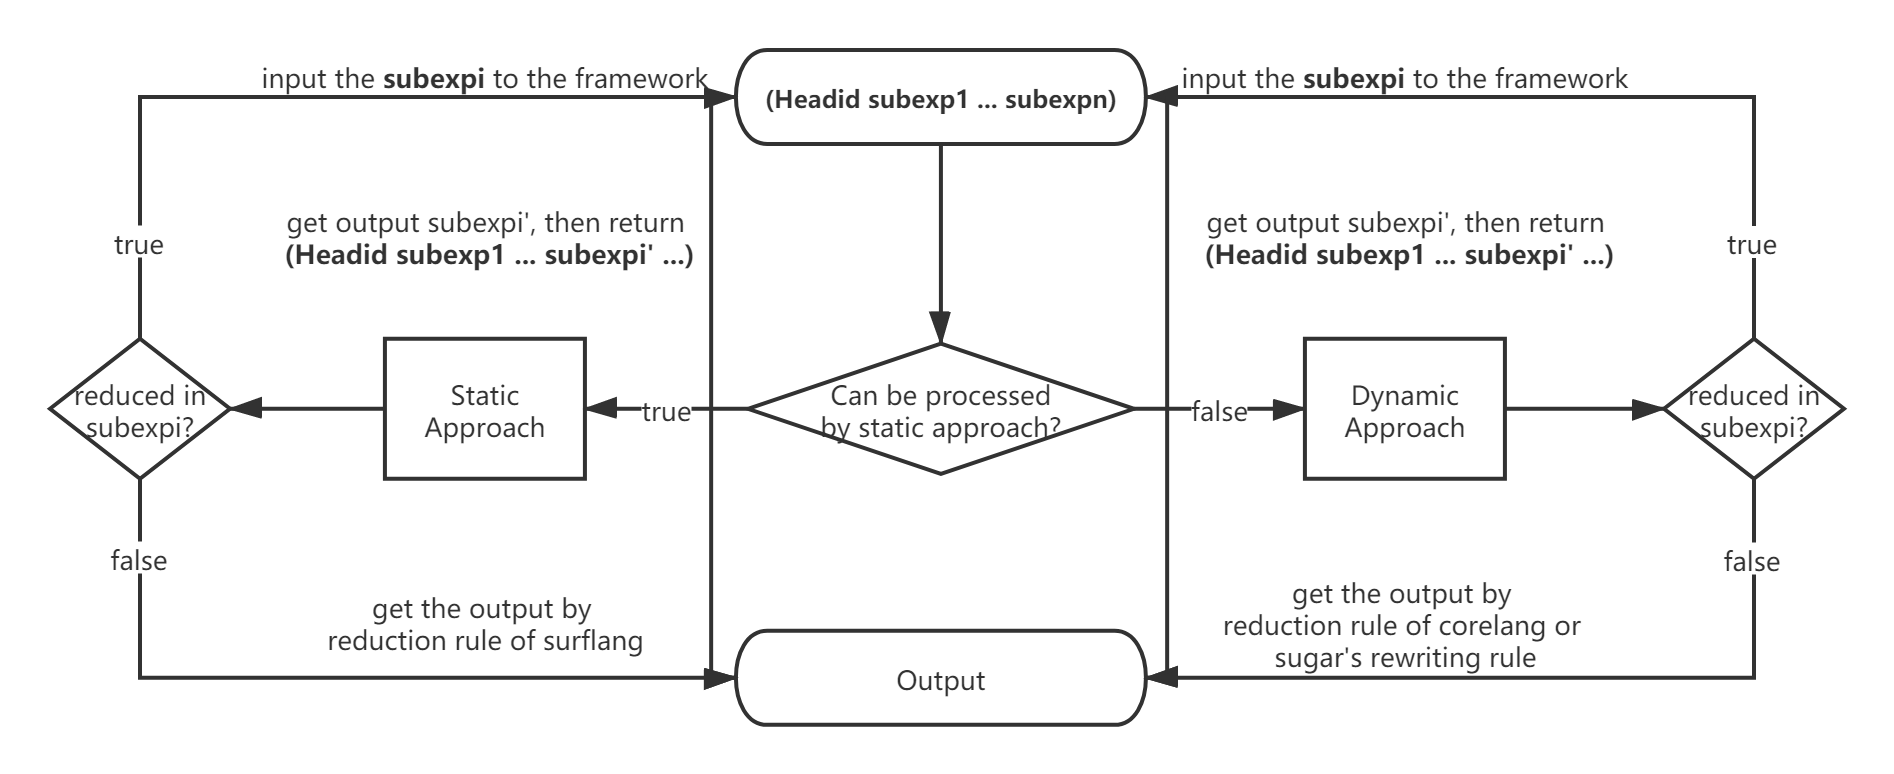
\includegraphics[width=12cm]{images/mixture.png}
    \caption{One step in framework of mixture approach}
    \label{fig:mixture}
\end{figure}

Given an example based on the former section. Besides sugar {\bfseries and}, {\bfseries or}, we add a recursive sugar {\bfseries mapf} based on another new sugar {\bfseries f}. The recursive sugar can be handled by the dynamic approach, but not for the static one. (Reasons in later sections)
\begin{Codes}
\small{(f e1 e2)} \DeStep{ (let x e1 (or x (and e2 x)))}
\small{(mapf e lst)} \DeStep{ (if (empty? lst) empty (cons (f e (first lst)) (mapf e (rest lst))))}
\end{Codes}

In the mapf (map of f) sugar, we use both core language's term (such as {\bfseries if, empty?, cons, let, first, rest}) and existing syntactic sugar ({\bfseries and, or}). The semantics of core language is as common. But to show some exact steps, we set the term {\bfseries cons} as a common expression (belonging to core language, but being displayed as surface language).


If we execute
\begin{Codes}
(mapf \#t (list \#f \#t))
\end{Codes}
 the mixture approach will judge whether sugar mapf can be handle by the static approach. No, then we use the dynamic approach in one step and get the intermediate expression.
\begin{Codes}
    (mapf \#t (list \#f \#t))
\OneStep{ (cons (f \#t (first (list \#f \#t))) (mapf \#t (rest (list \#f \#t))))}
\end{Codes}
Then according to semantics of {\bfseries cons}, the first subexpression should be reduced. The subexpression can be handled by the static approach, so getting a subsequence.
\begin{Codes}
    (cons (f \#t (first (list \#f \#t))) (mapf \#t (rest (list \#f \#t))))
\OneStep{ (cons (f \#t \#f) (mapf \#t (rest (list \#f \#t))))}
\OneStep{ (cons \#t (mapf \#t (rest (list \#f \#t))))}
\end{Codes}
Then the second subexpression should be reduced, which is a recursive process. Finally, the subexpression (mapf \#t (list)) will be processed by dynamic approach.
\begin{Codes}
   (mapf \#t (list))
\DeStep{ (if (empty? (list)) empty ...)}
\OneStep{ empty}
\end{Codes}
Note that there are some steps should not be displayed, we define the common expressions above in syntaxes to restrict which intermediate step should be displayed.
}

To solve the problem in the traditional approach, we propose a new resugaring approach by eliminating "reverse desugaring" via "lazy desugaring", where a syntactic sugar will be desugared only when it is necessary. We test the necessity of desugaring by a one-step try. We shall first briefly explain our one-step try resugaring method, and then show that how the "one-step try" can be cheaply done by derivation of evaluation rules for syntactic sugars.

\begin{Codes}
    (resugar (and (or \#t \#f) (and \#f \#t)))
\DeStep{\quad \note{ \{ a one-step try on the outermost and \}}
    (try (if (or \#t \#f) (and \#f \#t) \#f))}
\OneStep{\quad \note{\{ should reduce on subexpression (or \#t \#f) of and, delay desugaring of and\} }
    (and (resugar (or \#t \#f)) (and \#f \#t))} \note{// no reduction}
\DeStep{\quad \note{ \{ a one-step try on or \}}
    (and (try (if \#t \#t \#f)) (and \#f \#t))}
\OneStep{\quad \note{\{ keep this try, finish inner resugaring, and return to the top \}}
    (resugar (and \#t (and \#f \#t)))}
\DeStep{\quad \note{ \{ a one-step try on the outermost and \}}
    (try (if \#t (and \#f \#t)))}
\OneStep{\quad \note{\{ keep this try, finish inner resugaring, and return to the top \}}
    (resugar (and \#f \#t))}
\DeStep{\quad \note{ \{ a one-step try on the outermost and \}}
    (try (if \#f \#t \#f))} \note{// have to desugar and reduce}
\OneStep{ \#f}
\end{Codes}

For each step in the above, we make one reduction step and move resugaring focus if desugaring is unnecessary. So $7$ reduction steps are needed for our whole resugaring, while the traditional approach needs $9$ steps ($3$ in desugaring, $3$ in evaluation, $3$ for reverse resugaring). Note that reverse desugaring is more complex and costive because of match and substitution. Note also that the traditional approach would be more redundant if it works on larger expressions.
%As there is no need for tagging and reverse desugaring, our approach becomes lightweight.

We can go further to make our approach more efficient. As the purpose of a "one-step try" is to determine the computation order of the syntactic sugar, we should be able to derive this computation order through the desugar rules and the computation orders of the core language, rather than just through runtime computation of the core expression as done in the above. As will be shown in Section \ref{sec:ruleDerivation}, we can automatically derive evaluation rules (consist of the context rules and reductions rules) for both \emph{and} sugar and \emph{or}.
\[
\begin{array}{c}
\infer {(\mbox{and}~e_1~e_2) \rightarrow (\mbox{and}~e_1'~e_2)} {e_1~ \rightarrow~e_1'}
\qquad
(\mbox{and}~\#t~e2) \rightarrow e_2
\quad
(\mbox{and}~\#f~e2) \rightarrow \#f \\
\\
\infer {(\mbox{or}~e_1~e_2) \rightarrow (\mbox{or}~e_1'~e_2)} {e_1~ \rightarrow~e_1'}
\qquad
(\mbox{or}~\#t~e2) \rightarrow \#t
\quad
(\mbox{or}~\#f~e2) \rightarrow e_2 \\
\end{array}
\]
Now with these rules, our resugaring will need only $4$ steps.
\begin{Codes}
    (and (or \#t \#f) (and \#f \#t))
\OneStep{ (and \#t (and \#f \#t))}
\OneStep{ (and \#f \#t)}
\OneStep{ \#f}
\end{Codes}

Two remarks are worth making here. First, we do not require a complete set of reduction/context rules for all syntactic sugars; if we have these rules, we can elaborate them to remove one-step try, and make a shortcut for a sequence of evaluation steps on core expression.
For example, suppose that we have another syntactic sugar named \emph{hard} whose evaluation rules cannot be derived.
We can still do resugaring on \Code{(and (hard (and \#t \#t) ...) ...)}, as we do early.
Second, our example does not show the case when a surface expression contains language constructs of the core expression. This does not introduce any difficulty in our method, as we have no reverse desugaring, so there is no worry about desugaring an original core expression to a syntactic sugar. For instance, we can deal with \Code{(and (if \#t then (and \#f \#t) \#f) \#f)}, without resugaring it to \Code{(and (and \#t (and \#f \#t) \#f)}.


\subsection{New Features}

As will be seen clearly in the rest of this paper, our approach has the following new features.
\begin{itemize}
  \item {\em Efficient}. As we do not have "tagging" and costive and repetitive "reverse desugaring", our approach is much more efficient than the traditional approach. As discussed above, by deriving reduction/context rules for the syntactic sugars, we can gain more efficiency.

  \item {\em Powerful}. As we do not have "reverse desugaring", we can avoid complicated matching when we want to deal with local bindings (hygienic sugars) or more involved recursively defined sugars (see \Code{map} in Section \ref{sec:recursiveSugar}).

  \item {\em Lightweight}. Our approach can be cheaply implemented using the PLT Redex tool \cite{SEwPR}. This is because our "lazy" desugaring is much more simpler than "reverse desugaring" that needs careful design of patterns, and matching/substitution algorithms.

\end{itemize}
